\subsection{Reciprocal projection, feedback, and a recurrence waiting time}\label{sec:reciprocal}
The one-way projection result extends to a pair of calibrated populations. The new question is whether content sent in one direction can return in a direction that the first population reads. This requires a product of maps, not merely two individually nonzero maps. We derive both the carrier response and a time-domain threshold prediction from the same delayed feedback architecture. All maps and gains in this subsection are frozen; gain probes are externally calibrated rather than generated by the content feedback.

Let $P(t)\in\R^{n_P}$ and $Q(t)\in\R^{n_Q}$ be regional content features, where $n_P,n_Q$ are their feature dimensions, with independently timed external inputs $b_P,b_Q$. Absorb fixed positive gates and pathway weights into $L_{PQ}:\R^{n_Q}\to\R^{n_P}$ and $L_{QP}:\R^{n_P}\to\R^{n_Q}$. The first subscript denotes the receiver. These are the same operators as Section~\ref{sec:delayed}, closed into a reciprocal system, rather than a second unrelated model. For normalized causal processing kernels $h_f,h_b$, define
\begin{align}
(\mathcal L_f Q)(t)&=\int_0^\infty h_f(s)L_{PQ}Q(t-\tau_f-s)\,ds,\nonumber\\
(\mathcal L_b P)(t)&=\int_0^\infty h_b(s)L_{QP}P(t-\tau_b-s)\,ds.\label{eq:loop-operators}
\end{align}
The full loop is $P=b_P+\mathcal L_fQ$, $Q=b_Q+\mathcal L_bP$. On bounded signals, normalized nonnegative kernels give $\|\mathcal L_f\|\le\|L_{PQ}\|$ and $\|\mathcal L_b\|\le\|L_{QP}\|$. The product-norm condition below therefore makes the composite feedback operator a contraction, with solution
\[
P=(I-\mathcal L_f\mathcal L_b)^{-1}(b_P+\mathcal L_fb_Q)
=\sum_{k\ge0}(\mathcal L_f\mathcal L_b)^k(b_P+\mathcal L_fb_Q).
\]
This follows by substitution and convergence of the operator-norm geometric series. A return traverses both maps and both processing kernels. Their Fourier transforms multiply the corresponding carrier operators; time-domain echoes can consequently be dispersed rather than sharp jumps.

The discrete-delay equations used for the explicit latency result set each processing kernel to a unit point mass at zero. A point mass is not an integrable density under Section~\ref{sec:delayed}'s stated assumptions; it is an ideal limiting case. For example, the densities $h_\epsilon(s)=\epsilon^{-1}\mathbf{1}_{[0,\epsilon]}(s)$ satisfy those assumptions and concentrate at zero. For bounded continuous $Q$,
\begin{align*}
&\left\|\int h_\epsilon(s)L_{PQ}Q(t-\tau_f-s)\,ds-L_{PQ}Q(t-\tau_f)\right\|\\
&\qquad\le\|L_{PQ}\|\sup_{0\le s\le\epsilon}\|Q(t-\tau_f-s)-Q(t-\tau_f)\|\longrightarrow0.
\end{align*}
The analogous statement holds on the reverse edge. On bounded uniformly continuous signals this convergence is uniform in time; the common contraction bound then also gives convergence of the loop solutions through the resolvent identity. For step inputs, convergence is asserted away from discontinuities, not at the jump itself. Thus the sharp echo and integer-round-trip formula is a special instantaneous-processing limit; finite processing kernels require the convolutional first-passage calculation. In that limit specify
\begin{align}
P(t)&=b_P(t)+L_{PQ}Q(t-\tau_f),\nonumber\\
Q(t)&=b_Q(t)+L_{QP}P(t-\tau_b),\qquad \tau_f,\tau_b\ge0,\quad T_{\rm loop}=\tau_f+\tau_b>0.\label{eq:reciprocal}
\end{align}
The constant maps are translated receiver features, not raw anatomical connectivity. We use the sufficient stability condition $\|L_{PQ}\|\|L_{QP}\|<1$. General processing kernels would spread the echoes; their unknown phases and durations cannot be absorbed into an asserted conduction estimate.

\begin{theorem}[Reciprocal projected delivery and return support]\label{thm:reciprocal}
Assume Eq.~\eqref{eq:reciprocal}, zero prehistory, $b_P=0$, and a source step $b_Q(t)=d\,\mathbf{1}_{t\ge0}$. Write $A=L_{PQ}L_{QP}$. Then
\begin{equation}
P(t)=\sum_{k\ge0} A^k L_{PQ}d\,
\mathbf{1}_{t\ge\tau_f+kT_{\rm loop}}.\label{eq:echo}
\end{equation}
For a fixed readout $v$, the isolated $k$th increment is nonzero exactly when $v^\top A^kL_{PQ}d\ne0$. Direct projected delivery requires $v^\top L_{PQ}d\ne0$; an effective first return requires the additional condition $v^\top L_{PQ}L_{QP}L_{PQ}d\ne0$. The set of potentially delivered receiver features is contained in
\[
\mathcal S_d=\operatorname{span}\{L_{PQ}d,AL_{PQ}d,A^2L_{PQ}d,\ldots\}.
\]
A readout orthogonal to $\mathcal S_d$ never receives this item through the specified loop. At long times, $P(t)$ converges to $(I-A)^{-1}L_{PQ}d$.
\end{theorem}
\begin{proof}
Substitution of the second equation into the first gives
\[
P(t)=L_{PQ}d\,\mathbf{1}_{t\ge\tau_f}+A P(t-T_{\rm loop}).
\]
Before $\tau_f$ the forcing is zero and zero prehistory yields $P=0$. On $[\tau_f,\tau_f+T_{\rm loop})$ the delayed term still vanishes, so $P=L_{PQ}d$. Suppose the formula holds up to the $m$th interval. On the next interval, substituting its previous-interval value adds the term $A^{m+1}L_{PQ}d$ to the accumulated sum. Induction proves Eq.~\eqref{eq:echo}; for each finite time only finitely many terms are active because $T_{\rm loop}>0$. This also establishes the unique causal solution by the method of steps.

Subtracting the left limit from the value at $\tau_f+kT_{\rm loop}$ gives precisely $A^kL_{PQ}d$. Application of the linear functional $v^\top$ proves the increment criterion, including the direct and first-return cases. Every partial sum belongs to $\mathcal S_d$, so an orthogonal readout is identically zero. The bound $\|A\|\le\|L_{PQ}\|\|L_{QP}\|<1$ makes the infinite series absolutely convergent, since $\|A^kL_{PQ}d\|\le\|A\|^k\|L_{PQ}d\|$. Multiplying its partial sums by $I-A$ yields $L_{PQ}d-A^{m+1}L_{PQ}d$, whose last term tends to zero. Therefore the limit is $(I-A)^{-1}L_{PQ}d$. This argument concerns step responses of the stated stable model; it makes no claim that arbitrary matrix feedback increases every readout.
\end{proof}

\paragraph{Why two nonzero pathway maps are insufficient.} Take $L_{PQ}=\operatorname{diag}(1/2,0)$, $L_{QP}=\operatorname{diag}(0,1/2)$, and $d=v=e_1$. Both maps are nonzero, and the forward contribution is $1/2$, but $L_{QP}L_{PQ}d=0$: this item produces no return. Moreover, signed echo increments can cancel in a summed readout. Individually timed increments, rather than the nonzero status of each anatomical pathway, are the appropriate test of the product condition.

\begin{corollary}[An explicit recurrence contribution to completion latency]\label{cor:recurrence}
Suppose the delivered vector $p_0=L_{PQ}d$ lies in an invariant channel $Ap_0=\beta p_0$, with $a=v^\top p_0>0$ and $0\le\beta<1$. Define completion as the first time the signed readout reaches $\theta>0$. Then the readout on the $m$th interval is $a\sum_{k=0}^{m}\beta^k$. If $\theta\le a$, completion occurs at $\tau_f$. If $\beta=0$ and $\theta>a$, it never occurs. For $0<\beta<1$ and $a<\theta<a/(1-\beta)$,
\begin{align}
m_*&=\min\left\{m\in\{0,1,\ldots\}:\frac{a(1-\beta^{m+1})}{1-\beta}\ge\theta\right\},\nonumber\\
t_*&=\tau_f+m_*T_{\rm loop}.\label{eq:recurrence-latency}
\end{align}
If $\theta\ge a/(1-\beta)$ in this latter case, no finite completion occurs. A zero initial projected vector remains zero under the linear loop.
\end{corollary}
\begin{proof}
The eigenvector condition implies $A^kp_0=\beta^kp_0$ for every $k$ by induction. Apply $v^\top$ to Eq.~\eqref{eq:echo}. For $\beta=0$ the only nonzero increment is the first, proving the stated cases. For $0<\beta<1$ the partial sums increase strictly to $a/(1-\beta)$, so any threshold strictly between $a$ and that limit has a smallest finite crossing index. The series formula yields Eq.~\eqref{eq:recurrence-latency}. Each plateau begins with an attained right-continuous jump, so the first crossing is attained here without invoking the continuous-gain assumption of Corollary~\ref{cor:completion}. Every finite partial sum is strictly below its limit; equality with the limit therefore does not produce a finite crossing. If $p_0=0$, all powers of $A$ applied to it are zero. A zero direct scalar readout alone does not imply this last conclusion: feedback can rotate a nonzero vector into the readout at a later echo.
\end{proof}

With known source onset and resolved sharp increments, the first increment identifies $\tau_f$ and successive spacing identifies $T_{\rm loop}$, hence $\tau_b=T_{\rm loop}-\tau_f$. This constraint requires the instantaneous-processing limit and separation from measurement artifacts; finite unknown processing invalidates the direct conduction interpretation.

The additional term $m_*T_{\rm loop}$ is a derived accumulation waiting time. Projection and gates determine $a$ and $\beta$; conduction determines the spacing of successive opportunities. For $a=0.2$, $\beta=0.5$, $\tau_f=18$ ms, $\tau_b=12$ ms, and $\theta=0.34$, the readout steps through $0.2$, $0.3$, and $0.35$, crossing at 78 ms. This is 60 ms later than direct arrival. The same nonzero projection never reaches a threshold of $0.4$ at finite time. These examples replace the unsupported inference that nonzero projection ensures finite lag. The recurrence waiting time is distinct from the changing-phase waiting time in Section~\ref{sec:unreported-delay}; neither is an inferred universal duration of unreported processing.

\paragraph{Beyond an invariant channel.} Corollary~\ref{cor:recurrence} gives a closed scalar formula because all increments point in the same direction. General stable maps can rotate, cancel, or transiently amplify a readout. Their completion criterion is still explicit as a sequence of matrix partial sums, with a quantitative bound on the unresolved tail.

\begin{proposition}[General projected first passage and finite certification]\label{prop:generalpassage}
Under Theorem~\ref{thm:reciprocal}, put $p_0=L_{PQ}d$, let $v$ be a fixed readout, and set $q_A=\|A\|<1$. Define
\[
z_m=v^\top\sum_{k=0}^{m}A^kp_0,
\qquad z_\infty=v^\top(I-A)^{-1}p_0,
\qquad E_m=\frac{\|v\|\|p_0\|q_A^{m+1}}{1-q_A}.
\]
For a positive signed threshold $\theta$, the first attained event is $\tau_f+m_*T_{\rm loop}$, where $m_*=\min\{m\ge0:z_m\ge\theta\}$, or it never occurs if this set is empty. The tail satisfies $|z_\infty-z_m|\le E_m$. If $z_\infty>\theta$, completion is necessarily finite; any $m$ with $E_m<z_\infty-\theta$ is an upper bound on the crossing index. If all values through $M$ are below threshold and $z_\infty+E_M<\theta$, completion never occurs. Values $z_\infty\le\theta$ alone do not exclude an earlier transient crossing. For $n_P$ receiver coordinates, the readout is identically zero if and only if $v^\top A^kp_0=0$ for $k=0,\ldots,n_P-1$.
\end{proposition}
\begin{proof}
Equation~\eqref{eq:echo} is constant on each interval between consecutive return times, including its attained left endpoint. Applying $v^\top$ gives $z_m$ on the $m$th interval, proving the minimum-index rule without an invariance or positivity assumption. Absolute convergence yields
\[
|z_\infty-z_m|\le\|v\|\sum_{k=m+1}^{\infty}\|A\|^k\|p_0\|
=E_m.
\]
Since $E_m\to0$, if $z_\infty>\theta$ there is a finite $m$ with $z_m\ge z_\infty-E_m>\theta$. The first crossing is no later than this index. If $q_A=0$, the tail is zero and the first partial sum is already the limit. For every $m\ge M$, $E_m\le E_M$, so $z_m\le z_\infty+E_M<\theta$ certifies exclusion of all later crossings after the finite checked prefix. Equality in either bound does not provide the corresponding strict certification.

An identically zero readout has zero successive differences, so every $v^\top A^kp_0$ vanishes. Conversely, the Cayley--Hamilton identity expresses $A^{n_P}$ as a linear combination of lower powers. Multiplication by further powers and induction express all higher powers using $I,A,\ldots,A^{n_P-1}$. If the first $n_P$ scalar coefficients vanish, all subsequent ones vanish, and so does every partial sum. This proves the finite support test. None of these arguments requires $p_0$ to be an eigenvector.
\end{proof}

For example, take $A=\left(\begin{smallmatrix}0&0.5\\-0.5&0\end{smallmatrix}\right)$ and $p_0=v=e_1$. The first readout is 1, while its limit is 0.8; threshold 0.9 is crossed at direct arrival despite lying above the limit. Threshold 0.8, equal to the limit, is also crossed at direct arrival. Thus the scalar invariant-channel exclusion at equality is not general. With $p_0=e_1$, $v=e_2$, and $A=\left(\begin{smallmatrix}0&0\\0.5&0\end{smallmatrix}\right)$, the direct readout is zero and the first return is 0.5. Rotation into a readout can therefore create a later contribution even without scalar accumulation. For absolute-amplitude completion, replace $z_m\ge\theta$ by $|z_m|\ge\theta$; the same tail bound applies with $|z_\infty|$, while the signed example and minimum must be evaluated with the chosen rule.

\paragraph{Non-normal loops: contraction versus stability.} The Euclidean bound in Proposition~\ref{prop:generalpassage} can be conservative, but $\|A\|_2<1$ itself excludes growth of $\|A^kp_0\|_2$. A readout can nevertheless rise as the vector rotates. Genuine transient vector amplification requires a broader condition. The relevant extension is Schur stability, $\rho(A)<1$, where $\rho$ denotes the largest eigenvalue modulus. An $\varepsilon$-pseudospectrum describes sensitivity to perturbations and depends on $\varepsilon$; it is not a substitute for the norm bound used above.

\begin{proposition}[Stable non-normal return certification]\label{prop:stable-returns}
Retain the sharp-delay loop, zero prehistory, and step input of Theorem~\ref{thm:reciprocal}, but replace its product-norm condition by $\rho(A)<1$. The echo formula, finite Krylov support test, and first-passage rule still hold. Define
\[
G_A=\sum_{k=0}^{\infty}(A^k)^\top A^k,
\qquad q_G=\sqrt{1-1/\lambda_{\max}(G_A)}<1.
\]
This positive-definite matrix solves $G_A-A^\top G_AA=I$. With $\|p\|_G=\sqrt{p^\top G_Ap}$ and dual readout norm $\|v\|_{G^{-1}}=\sqrt{v^\top G_A^{-1}v}$, replace the Euclidean tail by
\begin{equation}
|z_\infty-z_m|\le
\|v\|_{G^{-1}}\|p_0\|_G\frac{q_G^{m+1}}{1-q_G}.
\label{eq:lyapunov-tail}
\end{equation}
All strict crossing/exclusion certificates in Proposition~\ref{prop:generalpassage} apply with this bound. Euclidean transient amplification is permitted.
\end{proposition}
\begin{proof}
Method-of-steps induction establishes the finite-time echo formula without any stability condition. For a finite matrix with $\rho(A)<1$, its Jordan form implies $\|A^k\|\le Cr^k$ for some $C<\infty$ and $\rho(A)<r<1$: each Jordan-block power is bounded by a finite polynomial in $k$ times its eigenvalue powers, and the polynomial is absorbed by the strictly larger exponential rate $r$. Nilpotent blocks vanish after finitely many powers. The series defining $G_A$ therefore converges absolutely. Its $k=0$ term is $I$, so $G_A\succeq I$ and is positive definite. Removing that term and shifting the convergent series proves the displayed Lyapunov identity.

For every vector $p$,
\[
\|Ap\|_G^2=\|p\|_G^2-\|p\|_2^2
\le(1-1/\lambda_{\max}(G_A))\|p\|_G^2.
\]
Thus the induced $G_A$ norm contracts by $q_G<1$. Cauchy--Schwarz after inserting $G_A^{1/2}$ and $G_A^{-1/2}$ gives $|v^\top p|\le\|v\|_{G^{-1}}\|p\|_G$. Applying this to the geometric tail yields Eq.~\eqref{eq:lyapunov-tail}. If $q_G=0$, the inequality forces $A=0$ and the tail is zero. The same convergent geometric-series identity gives $z_\infty=v^\top(I-A)^{-1}p_0$. Substitution of the new tail in the earlier strict certificates proves the claims. The finite support test uses Cayley--Hamilton alone and is unchanged. No normality, positivity, or scalar-channel assumption is needed.
\end{proof}

This is a standard Lyapunov construction applied to the paper's projected completion statistic. It extends the usable model class rather than introducing new stability mathematics. For
\[
A=\begin{pmatrix}0.65&1.2\\0&0.65\end{pmatrix},\quad
p_0=e_2,\quad v=e_1,
\]
$\rho(A)=0.65$ but $\|A\|_2>1$. The direct readout is zero; successive plateaus are $0$, $1.2$, $2.76$, $4.281$, and $5.5992$. Threshold $5$ is first reached on the fourth return, at 138 ms for the earlier 18/12 ms delays. The example's amplitudes are normalized illustrative output units. Supplementary Figure~S9 compares the actual tail with the certificate, and distinguishes Euclidean amplification from stability. Compute partial sums directly until a strict certificate is met; near equality, report unresolved status rather than treating a numerical tolerance as proof of crossing.


\paragraph{The same loop in the observation model.} At frequency $\Omega$, let the calibrated carrier operator on edge $e$ be
\[
K_e(\Omega,\psi_e)=g(\psi_e-\alpha_e-\Omega\tau_e)
e^{-i(\gamma_e+\Omega\tau_e)}M_e.
\]
Here $M_e$ is a fixed calibrated translation, and the transfer phase $\gamma_e$ remains distinct from receptive center $\alpha_e$. For the instantaneous real-map time-domain realization in Eq.~\eqref{eq:reciprocal}, $\gamma_e=0$; an unknown extra carrier transfer phase is an observation nuisance, not an additional delay in that step-response theorem. Known carrier processing factors can multiply $K_e$. Solving the two carrier equations gives
\begin{equation}
Y_P=(I-K_{PQ}K_{QP})^{-1}(B_P+K_{PQ}B_Q),\label{eq:loop-carrier}
\end{equation}
under $\|K_{PQ}\|\|K_{QP}\|<1$. This uses the same delayed map products as Eq.~\eqref{eq:echo}. It is a stationary carrier realization; a separately introduced frequency response must have a causal realization before it is used to predict broadband transients.

\begin{proposition}[Reciprocity alone does not resolve the single-band ridge]\label{prop:loop-ridge}
For fixed probes, maps, external input law, and parameter-independent observation noise, apply separately on either edge the admissible shift
\[
(\gamma_e,\alpha_e,\tau_e)\mapsto
(\gamma_e+\Omega u_e,\alpha_e+\Omega u_e,\tau_e-u_e).
\]
The complete stationary loop response and its observation law are unchanged. The six edge parameters consequently have at least two independent likelihood-null directions at one band. Time-resolved, independently anchored onsets and echoes need not inherit this invariance.
\end{proposition}
\begin{proof}
Both $\gamma_e+\Omega\tau_e$ and $\alpha_e+\Omega\tau_e$ remain unchanged on each edge. Therefore each complete $K_e$ remains unchanged, including its gain, and so do the product, inverse, and forcing in Eq.~\eqref{eq:loop-carrier}. Adding the fixed observation noise gives the same probability law. Differentiating the law along either edge shift gives zero score; the two shifts occupy disjoint parameter coordinates and are independent. Where regular Fisher information exists its rank is thus at most four. This is an upper bound, not a claim that every input or readout attains rank four. In contrast, Eq.~\eqref{eq:echo} contains $\tau_f$ in the first onset and $\tau_f+\tau_b$ in the spacing. Compensation of a phase at one frequency does not preserve these times. With known input onset, nonzero resolved increments, and known or absent processing, the first onset identifies $\tau_f$ and the spacing identifies the round-trip time, hence $\tau_b$. Missing or overlapping echoes remove that particular identifying argument.
\end{proof}

\paragraph{One model, two complementary tests.} Carrier calibration determines the gain and phase operators used to predict delivery; content perturbations and echo timing test those operators and provide transverse timing constraints that carrier observations alone lack. A matched reverse-path manipulation predicts a change in later echoes while the initial forward increment remains fixed. Learning changes the calibrated maps and hence the support and gain of the loop. The Gaussian readout below can be applied to a selected echo amplitude; the bilinear extension tests directions outside an independently calibrated additive response space. When feedback is present, that baseline must include its linear echo responses: feedback can itself rotate a feature into a previously silent readout. These are linked consequences and optional extensions of a common transfer architecture, rather than evidence that every assumption follows from the rank-one result.

\paragraph{Proposed prefrontal and interhemispheric application.} $P$ could be an independently localized prefrontal population and $Q$ a specified contralateral cortical population, with their report association measured separately. A hemisphere is not a single feature population, and prefrontal cortex is not assigned conscious status by anatomy. Prefrontal content decoding without volitional reports has been observed \citep{kapoor2022}; callosal delay estimates vary with axonal and pathway properties \citep{caminiti2013}. Neither study validates this loop model. Its test would calibrate both directed content maps, perturb each source independently, resolve the initial and returning increments, and assess Eq.~\eqref{eq:recurrence-latency} on held-out thresholds. The nonzero-projection criterion supports modeled communication between report-status populations, while the return-product criterion tests their reciprocal interaction. An additional physiological processing delay must be measured or modeled explicitly; it cannot be recovered from projection geometry alone.

\begin{figure}[htbp]\centering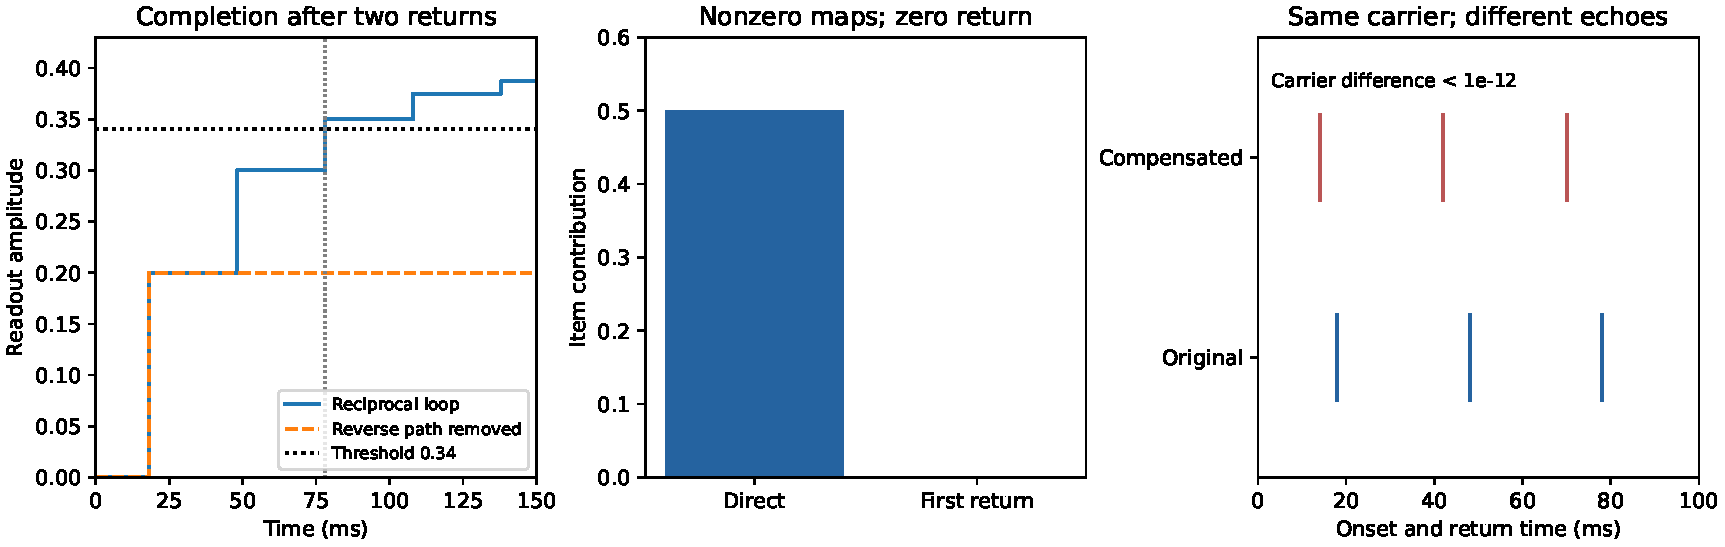
\includegraphics[width=.96\linewidth]{figure_reciprocal.pdf}\caption{Reproduced reciprocal-model checks. Left: positive aligned feedback reaches threshold after two returns; removing the reverse pathway preserves the first arrival but removes later increments. Middle: two nonzero maps can have a zero item-specific return product. Right: compensated edge parameters produce the same single-band carrier response but different directly anchored onset and echo times. Illustrative choices are $\tau_f=18$ ms, $\tau_b=12$ ms, direct amplitude $a=0.2$, return multiplier $\beta=0.5$, and threshold $\theta=0.34$.}\label{fig:reciprocal}\end{figure}
